\documentclass[12pt]{ctexart}
% set the left/right margin such that the main title can be written within one line
\usepackage[left=30mm]{geometry}
\usepackage{enumitem}
\AddEnumerateCounter{\chinese}{\chinese}{}
\usepackage{fancyhdr}
\usepackage{graphicx}
\usepackage{amssymb}
\usepackage{longtable}
\usepackage{hyperref}
\usepackage{subcaption}
\fancypagestyle{runningpage}
{
  \fancyhead{}
    \fancyhead[L]{
\includegraphics[height=12pt]{utsz_volunteer_org.jpg}} 
    \fancyhead[C]{深圳大学城志愿者部}
  \fancyfoot{}
  \fancyfoot[C]{第 \thepage 页}
}
% not works?
\ctexset {
 appendixname = {附录}
}
\def\CurriculumScheduleWidth{1.6cm}
\begin{document}
% first page is cover
\title{
    \vspace{-0.5in}
    \textmd{\textbf{\huge{2019寒假深圳大学城三校\\ 联合支教}}}\\
    \normalsize\vspace{0.1in}\Large{2018年秋季学期}\\
    \vspace{1in}
     \textbf{\huge{策}}\\
    \vspace{1in}
     \textbf{\huge{划}}\\
    \vspace{1in}
     \textbf{\huge{书}}\\
    \vspace{1in}
}
\author{策划人:李志超、赵丰、张晓冰}
\maketitle
\thispagestyle{empty}
\pagebreak
\pagestyle{runningpage}
\tableofcontents
% 为什么要联合5所高校?
% 实际:方便拉赞助
% ideal: 规模效应,影响力。

% 有没有能力组织,可行性如何?
% 退一万步说:即使没拉到赞助,志愿者车费全部自费也是比较吸引人的。毕竟其他支教队好多都无法报销车费的。有的,高校义工之间合作比较频繁。

% 能不能拿到官方支持?
% 难说。有利的一面是只是口头支持,不用官方掏钱。但既然官方出面,深圳这边媒体报道必须少不了。
% 不利的一面,人太多,不安全?
% 破:强调是一个松散的联盟。实际还是各高校自行组织。强调时代大背景:教育扶贫。深圳慈展会刚开完。

% 突破点:大公司的支持。腾讯公益啥的稍微支持一下就能把4万多的车费(60人)解决掉。
% 当地官方的支持也很重要。

% 短期支教弊端怎么破?
% 强调科学启蒙、寒假夏令营。

\section{项目背景}
深圳大学城志愿者部为深圳大学城片区六所高校义工组织形成的志愿组织联盟。

深圳大学城是全国唯一经国家教育部批准,由深圳地方政府联合著名大学共同举办,最初以培养研究生为主,云集了清华大学深圳研究生院、北京大学深圳研究生院、哈尔滨工业大学深圳研究生院。近年来随着哈尔滨工业大学深圳校区大规模扩建和开始招收本科生,深圳大学城在校生数量有了大幅增长。

%除了大学城三所高校外,在片区内还坐落着南方科技大学、中国科学院先进技术研究院以及深圳大学西丽校区。美丽的大沙河横穿六所高校校区。2018年秋季学期,通过深圳高校大型节水志愿活动、2018中国开源年会志愿服务以及南山区半程马拉松志愿服务等活动,六所高校的志愿组织密切协作,共同完成志愿者的招募和培训,活动的开展以及后期宣传等。
%本次联合支教即为六所高校志愿组织协商后一致同意的志愿项目。

大学生支教活动作为对国家偏远地区教育扶贫的一项有益补充,主要以本科生为主。以国家“西部计划”为号召,全国各大高校组织已保研的本科生和部分研究生每年会开展为期一年的长期支教活动。与长期支教相辅相成的是每年寒暑假开展的短期支教活动。短期异地支教活动
%由于要在孩子在放假的时候来学校上课,在偏远且交通不便的地方孩子的安全是个问题,且由于支教时间短,在传授文化课方面支教志愿者可能做得并不如当地教师好
目前在社会上受到一定的非议,部分原因是个别团队不够专业、不能因地制宜与当地志愿团队、当地家长、当地学校密切配合所致。


海南省“美在心灵”大学生支教志愿者协会在寒暑假与高校团队对接、共同组织开展在海南的支教活动由来以久。(或对接大学生支教联盟寒假支教的“童愿计划”,开展赴贵州等地的支教)

深圳市是一座年轻的城市,改革开放40年来,深圳市不仅在科技创新在全国名列全茅,在志愿服务领域的专业化程度也是走在全国的前列。“送人玫瑰、手有余香” 是深圳对外的一张名片。各行各业的“深圳人”利用自己的业余时间,发挥自己的所长帮助他人、回馈社会。

党的“十九大”以来,基层的脱贫攻坚作为基层工作的重点在全国推行。习总书记曾提出,“扶贫必扶智”。海南省XX市是国家重点扶贫单位。作为深圳高校的学生,我们希望能开拓志愿服务的思路,响应基层扶贫的号召,以“教育扶贫”为主题,深入当地开展支教活动。

我们希望在本次联合支教活动中可以进一步深入调研当地基础教育的建设情况,形成有价值的调研报告,在为当地基层教育事业作出切实贡献的同时,也能够为当地基础教育的长远发展提供参考。

\section{项目目标}
\begin{itemize}
\item 六所高校义工组织:扩大各高校志愿组织志愿服务的范围,进一步宣传自身组织等。
\item 参与者:体验短期支教生活,培养吃苦耐劳、乐于奉献的精神,形成对大学学习生活或科研生活的有益补充。
\item 支教地:提升支教地重视儿童教育的氛围,为当地基础教育的发展作出切实贡献。
\item 支教学生:打开孩子的视野,促进孩子的心灵成长。
\end{itemize}
\section{项目简介}
\begin{itemize}
\item 主办方:【需要挂名】
\item 承办方:
\begin{itemize}
\item 清华大学深圳研究生院紫荆志愿者团
\item 北京大学深圳研究生院青年志愿者协会
\item 哈尔滨工业大学深圳义工联合会
\end{itemize}
\item 地点:海南省XX市 XX小学、XX中学...
\item 时间:2019年1月XX日至2019年1月XX日,在支教地一周
\item 志愿者: 三所高校义工,共计30人
%\begin{table}[!ht]
%\centering
%\begin{tabular}{|c|c|c|c|c|}
%\hline
%姓名 & 性别 & 年级 & 系别 & 联系方式\\
%\hline
%赵丰 & 男 & 研一 & 电子系 & 18800190762 \\
%\hline
%张晓冰  &	男	& 研一 &  生物系 & 13938315159 \\
%\hline
%张炎武 & 男 & 研一 & 医院管理 & 18894000752\\
%\hline
%白杨 & 女 & 研一 & 电子系 & 18810913823\\
%\hline
%王鲜俐 & 女 & 研一 & 材料系 & 17633905356\\
%\hline
%黄少平 & 男 & 研一 & 自动化系 & 13696922357\\
%\hline
%周俞君(琼) & 女 & 大一 & 学前教育 & 13036084399 \\
%\hline
%周让强(琼) & 女 & 大二 & 医药营销 & 13518025473 \\
%\hline
%\end{tabular}
%\caption{参与支教志愿者名单}
%\end{table}
\end{itemize}
\section{项目实施方案}
\begin{enumerate}
\item 联络周边六所高校义工组织负责人,统一意见,获得各高校团委的同意。
\begin{enumerate}
\item 清华上届志愿团团长张晓冰 \checkmark
\item 大学城志愿者部李志超 \checkmark 
\item 北大青协王俊瑶 \checkmark 
\item 深大西丽校区义工联主席陈洁莲
\item 南科大义工联主席陈巍昱
\item 中科院义工队刘磊老师
\item 哈工大深圳义工联主席张伟明
\end{enumerate}
\item 确定主办方、支教地

寻求可以挂名的官方组织,首选南山共青团,但必须通过某高校团委【该高校团委作为牵头】官方发公函才能直接
对接到南山共青团;次选深圳大学城党委,这个相对比较简单。

确定好可以挂名的主办方即可与海南美在心灵对接(或联系其他基地),确定可以支教的市县。首选同一个市,且支教的中小学相对集中的地方。最低要求支教的市县能得到当地团委的口头支持【可以帮忙联系媒体、有领导可以出席开营仪式等】以及支教学校提供基本住宿保障。团委有物质上的支持最好,支教学校能承担部分餐饮费最好。

\item 寻求深圳当地企业赞助和支教地官方支持

\begin{enumerate}
\item 对接大学城周边餐饮店、文具店等\textbf{连锁} 机构;
\item 对接深圳市做中小学教育的机构,除常规赞助方案,外加可以帮忙对接校招(本科院校)、宣传招募兼职老师(特定企业),此处为赞助的大头,因为有些高校官方无法报销车费,以及餐饮费等;
\item 对接科技公司,希望将新产品带给支教地孩子开眼界、包括儿童机器人套装等。
\item 对接深圳的NGO、基金会等。
\end{enumerate}
\item 招募志愿者

六所高校义工组织分别招募志愿者组建支教队,研究生支队可与本科生支队分开。

\item 志愿者面试筛选、备课与筹备支教物资

\item 志愿者购买车票、出行保险
\end{enumerate}


\section{项目流程}
\begin{table}[!ht]
\centering
\begin{tabular}{|c|c|}
\hline
时间 & 安排 \\
\hline
 &  从深圳出发,经广州抵达海口 \\
\hline
 & 从海口东抵达XXX \\
\hline
 & 开营仪式\\
\hline
 & 日常支教活动,穿插家访、调研 \\
\hline
 & 结营仪式 \\
\hline
 & 志愿者返回 \\
\hline
\end{tabular}
\caption{行程安排表}\label{route}
\end{table}

%\begin{longtable}{|p{\CurriculumScheduleWidth}|p{\CurriculumScheduleWidth}|p{\CurriculumScheduleWidth}|p{\CurriculumScheduleWidth}|p{\CurriculumScheduleWidth}|p{\CurriculumScheduleWidth}|p{\CurriculumScheduleWidth}|p{\CurriculumScheduleWidth}|}
%\hline
%日期 & 7月30日 & 7月31日 & 8月1日 & 8月2日 & 8月3日 & 8月4日 & 8月5日 \\
%\hline
%& 星期一 & 星期二 & 星期三 & 星期四 & 星期五 & 星期六 & 星期天 \\
%\hline
%8:00-8:40  &  & 素质拓展(黄少平,大班)& 刮画(周俞君,大班)  & 孟母三迁(张炎武,大班)三字经(张晓冰,小班) & 材料科学(王鲜俐,大班)动物(张晓冰,小班)& 神话故事(白杨、大班)人文景观(周让强、小班) & 机械臂激光刻字(黄少平,大班)  \\
%\hline
%9:00-9:40 & &  素质拓展(黄少平,大班)& 中国地理(张炎武,大班) & 搭小车(赵丰,大班)刮画(周俞君,小班)  & 素质拓展(黄少平,大班)唱歌(周让强,小班) & 机械臂(黄少平,大班)古诗两首(张晓冰,小班) & 邦宝积木(赵丰,大班) \\
%\hline
%10:00-10:40 &  &  素质拓展(黄少平,大班) & &  搭小车(赵丰,大班)唱歌(周让强,小班)  &  素质拓展(黄少平,大班)折青蛙(张晓冰,小班)& 机械臂(黄少平,大班)千纸鹤(赵丰,小班)&    邦宝积木(赵丰,大班) \\
%\hline
%3:00-3:40  & 简单机械模型(赵丰,大班) &  &  &  &  &  & \\
%\hline
%4:00-4:40  & 遥控车模型(赵丰,大班) & &  &  &  & &  \\
%\hline
%\caption{旧洋村:课程表}\label{curriculum_schedule}
%\end{longtable}
%
%\begin{longtable}{|p{\CurriculumScheduleWidth}|p{\CurriculumScheduleWidth}|p{\CurriculumScheduleWidth}|p{\CurriculumScheduleWidth}|p{\CurriculumScheduleWidth}|p{\CurriculumScheduleWidth}|p{\CurriculumScheduleWidth}|p{\CurriculumScheduleWidth}|}
%\hline
%日期 & 7月30日 & 7月31日 & 8月1日 & 8月2日 & 8月3日 & 8月4日 & 8月5日 \\
%\hline
%& 星期一 & 星期二 & 星期三 & 星期四 & 星期五 & 星期六 & 星期天 \\
%\hline
%9:00-9:40 & 开营仪式 &   & &  & &  &   \\
%\hline
%3:00-3:40  &  & 折纸(王鲜俐,小班) &  简单机械模型(黄少平,大小班) & 素质拓展(黄少平,大班)千纸鹤(赵丰,小班) & 搭小车(赵丰,大班),动物世界(张晓冰,小班) & 趣味英语(周俞君,大班)人文景观(周让强) &  结营仪式 \\
%\hline
%4:00-4:40  &  & & 遥控车模型(赵丰,大小班)  & 素质拓展(黄少平,大班)刮画(周俞君,大班) & 搭小车(赵丰,大班),唱歌(周让强,小班) & 机械臂(黄少平,大班)体育(张晓冰,小班) & \\
%\hline
%\caption{打稔村:课程表}\label{curriculum_schedule}
%\end{longtable}

\section{项目后续阶段}
\begin{enumerate}
\item 整理资料,提交实践材料;完成往返火车票部分报销、出行保险报销;参与答辩等。
\item 借鉴“五彩石计划”或“旧洋关爱组”,对支教地的孩子给予持续的成长关注。
\end{enumerate}
\section{联系方式}
深圳大学城志愿者部:赵丰

Tel: 18800190762

Email: 616545598@qq.com

\begin{flushright}
深圳大学城志愿者部\\
\the\year 年 \the\month 月 \the\day 日
\end{flushright}

\begin{appendix}

\section{关于深圳大学城片区高校志愿组织}
\subsection{关于深圳大学城志愿者部}
深圳大学城志愿者部是在大学城社区党委的许可下,由深圳大学城片区六所高校组成的志愿组织联盟,为各类大型活动提供志愿服务。
\subsection{关于清华大学深圳研究生院紫荆志愿者团}
清华大学深圳研究生院紫荆志愿者服务团是清华大学深圳研究生院团委直属的学生志愿服务组织,以“自我实践、服务他人、自我教育、推动社会”为宗旨,旨在组织、协调我院研究生志愿者活动,开展具有清华特色的丰富多彩的研究生志愿活动。
\begin{figure}[!ht]
\centering
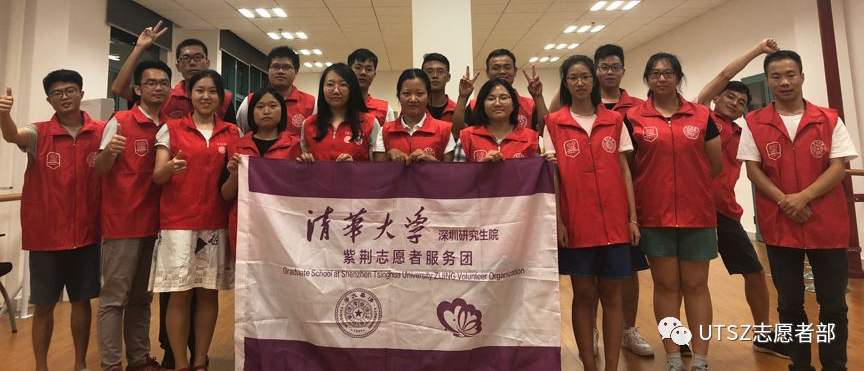
\includegraphics[width=14cm]{pic/zijing.png}
\end{figure}
2018年暑假,紫荆志愿团在海南省儋州市开展了支教扶贫系列活动,开拓了高校团队机器人支教的先河。


本次寒假清华大学深圳研究生院紫荆志愿者团拟开展的支教活动希望以成本价购入儿童机器人套装作为教具,发挥
自身专业优势开展支教活动。通过研究生寒假社会实践体系实现车费的报销。
%\begin{table}[!ht]
%\centering
%\begin{tabular}{|p{2cm}|p{2cm}|p{2cm}|p{3cm}|}
%\hline
%名称 & 来源 & 用途 \\
%\hline
%%深圳市搭搭乐乐文化传播有限公司
%儿童、初中机器人套装&  &  \\
%\hline
%素质拓展道具 & 心理辅导中心 &  \\
%\hline
%DOBOT魔术师(价值一万元) & 越疆科技 & \\
%\hline
%教具& &  \\
%\hline
%文具奖品 & & 课堂奖励 \\
%\hline
%\end{tabular}
%\caption{清华支教队所需教具参考}
%\end{table}

关于“旧洋关爱组”:旧洋村是一个支教点,紫荆团队和琼台师范学院2018年暑期在此支教。旧洋关爱组的实体是一个QQ群,由紫荆团队、琼台师范学院和支教地的孩子组成。各位支教老师利用自己的业余时间针对孩子暴露出的问题进行有针对性的疏导。紫荆团队在中秋佳节专程到东莞看望支教点的一个辍学的孩子,他现在跟着父母在莞城打工。
\begin{figure}[!ht]
\centering
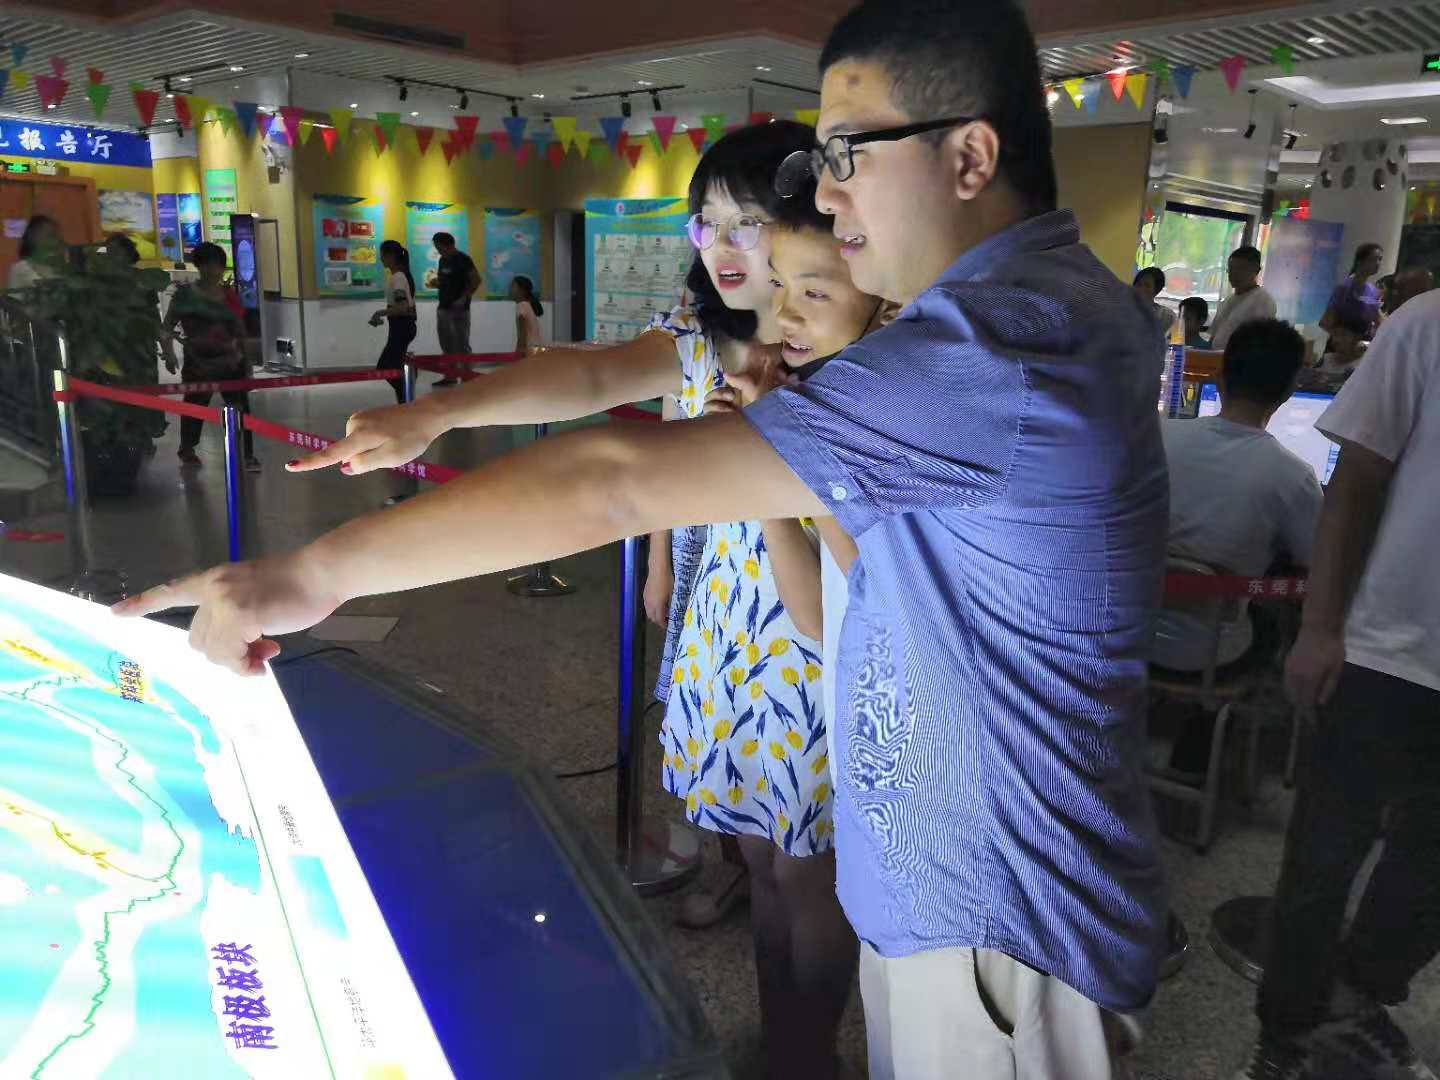
\includegraphics[width=12cm]{pic/zijing_talk.jpeg}
\caption{紫荆志愿者在东莞科技馆给孩子讲解}
\end{figure}
\subsection{关于北京大学深圳研究生院青年志愿者协会}
通过北京大学深圳研究生院研究生寒假社会实践自主立项的方式可进行支教立项,获得车费的报销。
\subsection{关于哈尔滨工业大学深圳义工联合会}
\begin{enumerate}
\item  \begin{itemize}
\item 支教地点:云南喜洲、云南洱源两所同维希望小学
\item 支教时间:2018年5月30日至6月10日
\item 合作单位:深圳市共进电子股份有限公司同维爱心公益基金会
\item 支教志愿者合影:
\begin{figure}[!ht]
\centering
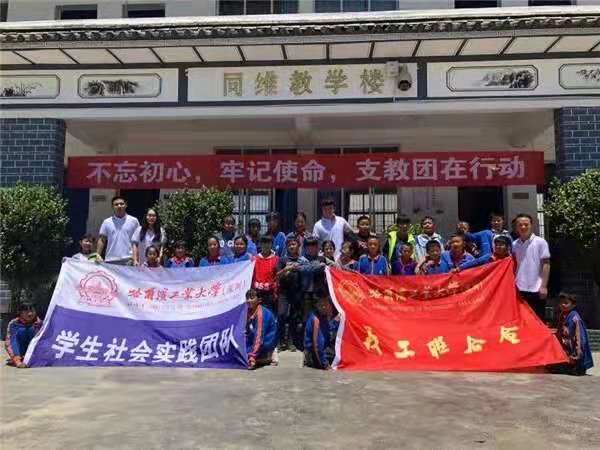
\includegraphics[width=12cm]{pic/hitsz_2018.jpeg}
\end{figure}
\end{itemize}
\item \begin{itemize}
\item 往期支教地点:江西省赣州市上犹县石坑希望小学
\item 支教时间: \begin{enumerate}
				\item 2013年7月7日至2013年7月23日 
				\item 2014年7月12日至7月26日
				\item 2015年7月4日至7月18日
				\item 2016年7月4日至2016年7月20日
			  \end{enumerate}
\item 支教志愿者合影:
\begin{figure}[!ht]
\centering
  \begin{subfigure}[b]{0.45\textwidth}
  
\includegraphics[width=\textwidth]{pic/hitsz_2015.png}  
        \caption{2015年 }
    \end{subfigure}~
      \begin{subfigure}[b]{0.45\textwidth}
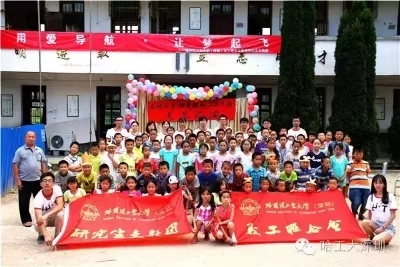
\includegraphics[width=\textwidth]{pic/hitsz_2016.jpeg}  
        \caption{2016年 }
    \end{subfigure}
\end{figure}
\end{itemize}
\end{enumerate}

关于“五彩石”计划:哈工大义工联合会2018暑假在云南两所希望小学支教,希望通过与支教地
的小朋友结对与书信往来的方式帮助山区的小朋友成长。目前该项目正在开展。
\section{关于美在心灵}
海南省“美在心灵”大学生支教志愿者协会(简称美在心灵)于2008年1月30日诞生于琼海市嘉积中学,2010年3月29日接受共青团海南省委业务主管,2011年7月11日在海南省民政厅注册成为合法民间公益机构,2017年12月6日被海南省民政厅授予“慈善组织”资格。美在心灵以“团结友爱,奉献社会”为宗旨,不以盈利为目的,广泛招募世界各地大学生志愿者到琼藏等乡村小学开展爱心支教活动,致力给孩子们一个快乐成长平台,给大学生一个社会实践机会,给社会一个务实且放心的爱心渠道,给政府一个温暖的辅助。目前已有美国、英国、俄罗斯、新加坡、韩国、日本等40多个国籍的大学生志愿者,以及清华、北大、港澳台等境内国内名校的大学生志愿者参加支教活动。十年以来,美在心灵安排志愿者1.9万人次,服务小学754所次(包括西藏两所小学:恩达小学和宾达小学),受益学生6.2万人次,总服务时长165万小时,总投入善款158万元。

\section{项目财务预算}\label{scheduling}
%所需物资具体到总共要多少钱


\begin{enumerate}
\item 往返车票:部分高校通过寒假实践流程可予以报销、部分需要由企业赞助或志愿者自费。单人单程350元左右。
\item 住宿费:由当地学校帮忙解决。由于购置生活必需品产生的开支单人单程50元左右。
\item 餐饮,部分由当地政府承担、部分由相关餐饮企业赞助费用、部分由志愿者自费。预估单人7天需要350元左右。
\item 教具(如机器人与科技产品等)与宣传资料:部分通过校团委报销、部分由相关文娱企业赞助。
\item 物资邮寄费用:部分由当地政府承担、部分需要由企业赞助。统一邮寄可节省开支,预估单程1000元。
\item 志愿者出行保险:部分高校通过寒假实践流程可予以报销、部分需要由企业赞助。单人7天需要20元左右。
\item 助学物资:企业赞助。
\end{enumerate}
按60人参与计算,预估总费用 7万元。
\section{赞助方案}
我们为赞助商设计了不同的合作方案以满足您多样化的需求。根据赞助金额的不同,我们初步设计了如下三个档位的赞助方案:
\begin{itemize}
\item 方案A——赞助4000元;
\item 方案B——赞助2000元; 
\item 方案C——赞助1000元。
\end{itemize}
不同赞助档位享受的宣传回报(见下表)有所不同,您可以根据自己的预算与想要实现的宣传力度选择合适的档位,如果这些都不能满足您的需要,具体的赞助金额以及赞助回报还可结合您的具体情况最终决定。目前初步拟定的赞助回报具体实施方案如下:
\begin{table}[!ht]
\centering
\begin{tabular}{|c|c|c|c|}
\hline
赞助方案 & 方案A & 方案B & 方案C \\
\hline
活动宣传 & \checkmark & \checkmark & \checkmark \\
\hline
现场鸣谢 & \checkmark &  \checkmark & \\
\hline
公众号文章宣传与转载 & \checkmark & &\\
\hline
活动冠名 & \checkmark & & \\
\hline
\end{tabular}
\end{table}

\begin{itemize}
\item 活动宣传:在各高校义工联公众号上的线上宣传中,均特殊标记鸣谢活动赞助商。
\item 现场鸣谢:在开营、闭营活动中,主持人鸣谢活动赞助商的大力支持。
\item 公众号文章宣传与转载:由支教队提供突出赞助商的文章,可由赞助商公众号进行转载。
\item 活动冠名:冠名赞助商以承办方。
\end{itemize}
备注:除了三种方案,我们欢迎有兴趣的商家赞助文具,高档食品等。如果商家有其他赞助需求,可以进一步商谈,定制方案。




\section{志愿者保障和守则}
\subsection{保障}
\begin{enumerate}
\item 志愿深圳平台工时。
\item 志愿者出行人身意外保险。
\item 住宿保障。
\item 一定额度的往返车费补贴和餐饮补贴。
\end{enumerate}
\subsection{守则}
\begin{enumerate}[label = {(\chinese*)}]
\item 具有完全民事行为能力的学生;
\item 认同紫荆志愿团理念和文化,尊重“美在心灵”的支教理念;
\item 服从支队长、村书记和相关爱心人士在支教期间的引导;
\item 有社会责任感和奉献精神,无不良嗜好;
\item 有较强的团结协作能力、语言表达能力和人际交往能力,尊重队友;
\item 有较强的心理素质,在艰苦的环境下能自我调节,保持积极乐观心态,肯吃苦,能坚持,不给支教项目及队友带来负面影响; 
\item 有爱心,热心帮助当地的学生和村民,尊重当地的民族文化和信仰;
\end{enumerate}
\end{appendix}
\end{document}

